% Intended LaTeX compiler: pdflatex
\documentclass[10pt,a4paper,UTF8]{article}
\usepackage{zclorg}
\author{张朝龙}
\date{}
\title{练习:可逆性与同构}
\hypersetup{
 pdfauthor={张朝龙},
 pdftitle={练习:可逆性与同构},
 pdfkeywords={},
 pdfsubject={},
 pdfcreator={Emacs 25.0.50.1 (Org mode 9.0.5)}, 
 pdflang={English}}
\begin{document}

\maketitle
\tableofcontents
\titlepic{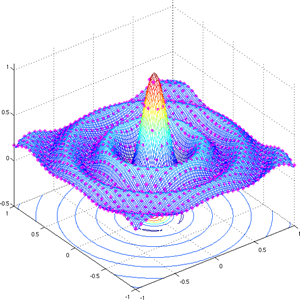
\includegraphics[scale=0.25]{../../img/sinc.PNG}}

\section{3.D.1}
\label{sec:org865dae5}


\begin{problem}
设\(T\in \mathcal{L}(U,V)\)和\(S\in \mathcal{L}(V,W)\)都是可逆的线性映射。证明\(ST\in \mathcal{L}(V,W)\)可逆且\((ST)^{-1} = T^{-1}S^{-1}\)
\end{problem}

\begin{answer}
根据3.56,可逆映射既是单的又是满的。

假设\(u,v\in U\),且\(STu = STv\)。根据\(S\)是单射,所以有\(Tu=Tv\);再根据\(T\)是单射,所以有\(u=v\).即,\(ST\)是单射。

令\(w\in W\),则有\(v\in V\)使得\(Sv=w\)(因为\(S\)是满射)。对于\(v\in V\),都有\(u\in U\)使得\(Tu=v\)。综上有对于任意的\(w\in W\)都有 \(STu = w\),所以\(ST\)是满射。

因为\(ST\)既是单射又是满射所以\(ST\)是可逆的。


因为\(ST(T^{-1}S^{-1}) = S(TT^{-1})S^{-1} = SS^{-1} = I\),且\(T^{-1}S^{-1}ST = T^{-1}T = I\)

所以有\(ST\)的逆映射是\(T^{-1}S^{-1}\)
\end{answer}

\section{3.D.2}
\label{sec:orgc490f0d}


\begin{problem}
设\(V\)是有限维的,且\(\dim V > 1\)。证明\(V\)上不可逆的算子构成的集合不是\(\mathcal{L}(V)\)的子空间。
\end{problem}

\begin{answer}
我们对\(\dim V = 2\)的例子给出反例。假设\(S,T\in \mathcal{L}(V)\),且有\(e_{1},e_{2}\)是\(V\)的标准基:
\[Te_{1} = 0;Te_{2} = e_{2}\]
\[Se_{1} = e_{1};Se_{2} = 0\]
因为\(nullT \neq \{0\}\),且\(nullS \neq \{0\}\),所以\(S,T\)都是不可逆映射。

所以有
\begin{eqnarray*}
(S+T)e_{1}&=&e_{1} \\
(S+T)e_{2}&=&e_{2}
\end{eqnarray*}

显然\(S+T\)是恒等映射,恒等映射是可逆映射。原命题得证。
\end{answer}

\section{3.D.3}
\label{sec:org1f0cab9}


\begin{problem}
设\(V\)是有限维的,\(U\)是\(V\)的子空间,且\(S\in \mathcal{L}(U,V)\)。证明:存在可逆的算子\(T\in \mathcal{L}(V)\)使得对每个\(u\in U\)均有\(Tu = Su\)当且仅当\(S\)是单射。
\end{problem}

\begin{answer}
首先因为\(T\)是\(\mathcal{L}(V)\)上的可逆算子,且满足\(Tu = Su\),所以\(S\)是单射,因为\(T\)是单射。


然后假设\(S\)是单射,设\(U\)的一个基是\(u_{1},\ldots ,u_{m}\),因为\(S\)是单的,则\(Su_{1},\ldots ,Su_{m}\)在\(V\)中也是线性独立的。我们把\(u_{1},\ldots ,u_{m}\)扩展成\(V\)的基:\(u_{1},\ldots ,u_{m},w_{1},\ldots ,w_{n}\);同样,我们也可以把\(Su_{1},\ldots ,Su_{m}\)扩展成\(V\)的基,\(Su_{1},\ldots ,Su_{m},e_{1},\ldots ,e_{n}\)

然后我们定义映射\(T:V\rightarrow V\)。满足:
\begin{equation}
\label{eq:1}
Tu_{i} = Su_{i},Tw_{j} = e_{j}, \quad 1 \leq i \leq m \quad 1 \leq j \leq n
\end{equation}
由于\(u_{1},\ldots ,u_{m}\)是\(U\)的一个基,所以可以保证上述定义\(T\)的唯一性。

对于任意的\(u=a_{1}u_{1} + \ldots + a_{m}u_{m}\),\(a_{i}\in \mathbf{F}\),我们有:
\begin{eqnarray*}
Tu&=&T(a_{1}u_{1} + \ldots + a_{m}u_{m}) \\
&=&a_{1}T(u_{1}) + \ldots + a_{m}T(u_{m}) \\
&=&a_{1}S(u_{1}) + \ldots + a_{m} S(u_{m}) \\
&=&S(a_{1}u_{1} + \ldots + a_{m}u_{m}) \\
&=&Su
\end{eqnarray*}

对于任意的\(v\in V\),都有:
\begin{equation}
\label{eq:2}
v = b_{1}u_{1} + \ldots + b_{m}u_{m} + c_{1}w_{1} + \ldots + c_{n}w_{n}
\end{equation}
对上式两边进行\(T\)映射,则有:
\begin{eqnarray*}
Tv&=&T( b_{1}u_{1} + \ldots + b_{m}u_{m} + c_{1}w_{1} + \ldots + c_{n}w_{n}) \\
&=&b_{1}Tu_{1} + \ldots + b_{m}Tu_{m} + c_{1}Tw_{1} + \ldots + c_{n}Tw_{n} \\
&=&b_{1}Su_{1} + \ldots + b_{m}Su_{m} + c_{1}e_{1} + \ldots + c_{n}e_{n}
\end{eqnarray*}
显然有:\(rangeT \subseteq V\)。

另外一方面\(Tu_{1},\ldots ,Tu_{m},Tw_{1},\ldots ,Tw_{n}\)包含于\(rangeT\) 所以 
\(span(Tu_{1},\ldots ,Tu_{m},Tw_{1},\ldots ,Tw_{n})\subseteq rangeT\)

所以\(T\)是满射。又因为3.69(对于有限维空间上的映射而言,满射意味着单射,意味着可逆映射),所以\(T\)是可逆映射。
\end{answer}


\section{3.D.4}
\label{sec:org0b0a1a3}


\begin{problem}
设\(W\)是有限维的,\(T_{1},T_{2}\in \mathcal{L}(V,W)\),证明:\(nullT_{1} = nullT_{2}\)当且仅当存在可逆的算子\(S\in \mathcal{L}(W)\)使得\(T_{1} = ST_{2}\)
\end{problem}

\begin{answer}
假设有\(nullT_{1} = nullT_{2}\),因为\(W\)是有限维的,所以\(rangeT_{2}\)也是有限维的。假设\(w_{1},\ldots ,w_{n}\)是\(rangeT_{2}\)的一个基,所以存在\(v_{1},\ldots ,v_{n}\in V\)使得\(T_{2}v_{i} = w_{i},i=1,\ldots ,n\),\(v_{1},\ldots ,v_{n}\)的存在性可以通过线性映射基本定理得到满足.

现在证明\(V = nullT_{2}\oplus span(v_{1},\ldots ,v_{n})\),对于任何\(v\in V\),存在\(a_{i}\in \mathbf{F},i \in \{1,\ldots ,n\}\)我们有:
\begin{equation}
\label{eq:3}
T_{2}v = a_{1}w_{1} + \ldots + a_{n}w_{n}
\end{equation}

因此有:
\begin{equation}
\label{eq:4}
T_{2}(v-a_{1}v_{1} -\ldots -a_{n}v_{n}) = 0
\end{equation}
也就是说:
\[v = (v-a_{1}v_{1} -\ldots -a_{n}v_{n})  + (a_{1}v_{1} + \ldots + a_{n}v_{n})\]
又因为\(v\)的任意性,所以:
\begin{equation}
\label{eq:5}
V = nullT_{2} + span(v_{1},\ldots ,v_{n})
\end{equation}
接下来我们证明直和的条件成立,即\(nullT_{2}\cap span(v_{1},\ldots ,v_{n}) = \{0\}\) 假设\(a_{1}v_{1} + \ldots + a_{n}v_{n} \in nullT_{2}\)我们有:
\begin{equation}
\label{eq:6}
T_{2}(a_{1}v_{1} + \ldots + a_{n}v_{n}) = a_{1}w_{1} +\ldots + a_{n}w_{n} = 0
\end{equation}

因为\(w_{1},\ldots ,w_{n}\)是线性无关的,所以\(a_{1},\ldots ,a_{n}\)都是零。所以:
\begin{equation}
\label{eq:7}
V = nullT_{2} \oplus  span(v_{1},\ldots ,v_{n})
\end{equation}

同样的,因为\(v_{1},\ldots ,v_{n}\)是线性无关的,所以\(T_{1}v_{1},\ldots ,T_{1}v_{n}\)也是线性无关的。又因为\(nullT_{1} = nullT_{2}\),所以有:
\begin{equation}
\label{eq:8}
0 = T_{2}(a_{1}v_{1} + \ldots + a_{n}v_{n}) = a_{1}w_{1} + \ldots +a_{n}w_{n}
\end{equation}

现在我们扩展两个\(W\)的基,一个从\(T_{1}v_{1},\ldots ,T_{1}v_{n}\)扩展到\(T_{1}v_{1},\ldots ,T_{1}v_{n},f_{1},\ldots ,f_{m}\),另一个从\(w_{1},\ldots ,w_{n}\)扩展到\(w_{1},\ldots ,w_{n},e_{1},\ldots ,e_{m}\)。在这两个基之间我们定义\(S\in \mathcal{L}(W)\)使得:
\begin{equation}
\label{eq:9}
Sw_{i} = T_{1}v_{i},Se_{j} = f_{j},i=1,\ldots ,n;j=1,\ldots ,m
\end{equation}
之前我们有\(V = nullT_{2} \oplus  span(v_{1},\ldots ,v_{n})\) 所以对于任何的\(v\in V\)可以写成:
\begin{equation}
\label{eq:10}
v = v_{null} + a_{1}v_{1} + \ldots + a_{n}v_{n}
\end{equation}
所以有:
\begin{eqnarray*}
ST_{2}(v)&=&ST_{2}(v_{null} + a_{1}v_{1} + \ldots + a_{n}v_{n}) \\
&=& ST_{2}(a_{1}v_{1} + \ldots + a_{n}v_{n}) \\
&=& S(a_{1}w_{1} + \ldots + a_{n}w_{n}) \\
&=&a_{1}T_{1}(v_{1}) + \ldots + a_{n}T_{1}(v_{n}) \\
&=&T_{1}(a_{1}v_{1} + \ldots + a_{n}v_{n}) \\
&=& T_{1}(v_{null} + a_{1}v_{1} + \ldots +a_{n}v_{n}) \\
&=& T_{1}(v)
\end{eqnarray*}
所以有\(ST_{2} = T_{1}\)。因为\(S\)是满射,因此\(S\)是单射。

另一方面假设存在可逆映射\(S\in \mathcal{L}(W)\)满足\(ST_{2} = T_{1}\),对于任何\(\mu \in nullT_{1}\),我们有:
\begin{equation}
\label{eq:12}
ST_{2}\mu = T_{1}\mu =0
\end{equation}
因为\(S\)是单射所以,其零空间等于\(\{0\}\),所以\(T_{2}\mu =0\),因此\(\mu \in nullT_{2}\)。所以\(nullT_{1} \subseteq nullT_{2}\),同样的,考虑到\(T_{2} = S^{-1}T_{1}\)我们有\(nullT_{2}\subseteq nullT_{1}\),所以有\(nullT_{1} = nullT_{2}\)
\end{answer}
\section{3.D.5}
\label{sec:orgf241725}


\begin{problem}
设\(V\)是有限维的,\(T_{1},T_{2}\in \mathcal{L}(V,W)\)。证明:\(range T_{1} = rangeT_{2}\)当且仅当存在可逆的算子\(S\in \mathcal{L}(V)\)使得\(T_{1} = T_{2}S\)
\end{problem}

\begin{answer}
我们假设\(rangeT_{1} = rangeT_{2}\),令\(u_{1},\ldots ,u_{m}\)是\(nullT_{1}\)的一个基,我们可以把这个基扩展为\(V\)的一个基\(u_{1},\ldots ,u_{m},w_{1},\ldots ,w_{n}\)。那么根据线性映射基本定理的证明过程我们有:\(rangeT_{1}=span(Tw_{1},\ldots ,Tw_{n})\),另外\(Tw_{1},\ldots ,Tw_{n}\)是线性独立的。因为\(rangeT_{1} = rangeT_{2}\)那么存在\(v_{1},\ldots ,v_{n}\in V\)使得\(T_{1}w_{i} = T_{2}v_{i},i= 1,\ldots ,n\)因为\(T_{1}w_{1},\ldots ,T_{1}w_{n}\)是线性独立的,那么\(T_{2}v_{1},\ldots ,T_{2}v_{n}\)也是线性独立的,所以\(v_{1},\ldots ,v_{n}\)也是线性独立的。由于\(rangeT_{1} = rangeT_{2}\),则有\(nullT_{1} = nullT_{2}\),令\(\zeta_{1},\ldots ,\zeta_{m}\)是\(nullT_{2}\)的一个基,那么\(\zeta_{1},\ldots ,\zeta_{m},v_{1},\ldots ,v_{n}\)是\(V\)的一个基。我们定义\(S\in \mathcal{L}(V)\),使得:
\begin{equation}
\label{eq:13}
Su_{i} = \zeta_{i} , \quad Sw_{j} = v_{j}
\end{equation}
那么我们有:
\begin{equation}
\label{eq:14}
T_{1}w_{j} = T_{2}v_{j} = T_{2}Sw_{j}, j = 1,\ldots ,n
\end{equation}
且:
\begin{equation}
\label{eq:15}
T_{1}u_{i} = 0 = T_{2}\zeta_{i} = T_{2}Su_{i} , i = 1,\ldots ,m
\end{equation}

因此\(T_{1} = T_{2}S\),因为我们定义\(S\)是在\(V\)的一个基上定义的,所以其唯一性得到保证。又因为\(S\)是满射,所以\(S\)是可逆的。

如果存在一个可逆线性映射\(S\in \mathcal{L}(V)\)使得\(T_{1} = T_{2}S\),那么对于\(\forall \mu \in V\)都有:
\begin{equation}
\label{eq:16}
T_{1}\mu = T_{2}S\mu \in range T_{2}
\end{equation}
所以\(rangeT_{1} \subseteq rangeT_{2}\)。

因为\(S\)是可逆的,所以\(T_{2}= T_{1}S^{-1}\),我们会得到\(rangeT_{2} \subseteq rangeT_{1}\).综上我们得到了\(rangeT_{1} = rangeT_{2}\)。

这个题目和上一个题目在证明过程中有些许类似,总结如下:
\begin{enumerate}
\item 都在一个空间上构建了两个基,并在这两个基之间构建了一个可逆映射。
\item 都用到了基于基构建的线性映射的唯一性。可见3.5非常重要。3.5告诉我们基于定义域的基构建的线性映射具有唯一性。
\item 都用到了3.22线性映射基本定理证明的过程。
\item 都用到了一个命题:假设\(T\in \mathcal{L}(V,W)\)且\(v_{1},\ldots ,v_{m}\)是\(V\)的一个向量组,满足\(Tv_{1},\ldots ,Tv_{m}\)是线性独立的,那么\(v_{1},\ldots ,v_{m}\)是线性独立的。证明过程很简单。值得注意的是这个问题反过来却不一定成立。即我们不能说\(v_{1},\ldots ,v_{m}\)是线性独立的,就说\(Tv_{1},\ldots ,Tv_{m}\)是线性独立的。因为:
\end{enumerate}
\begin{equation}
\label{eq:17}
a_{1}Tv_{1} + \ldots + a_{m}Tv_{m} = T(a_{1}v_{1} + \ldots + a_{m}v_{m}) = 0
\end{equation}
并不意味着\(a_{1}v_{1}+ \ldots + a_{m}v_{m}=0\)。因为有可能\(a_{1}v_{1}+ \ldots + a_{m}v_{m} \in nullT\) 。在线性映射基本定理3.22的证明过程中考虑到了这一个问题。
\end{answer}
\section{3.D.6}
\label{sec:org813592b}


\begin{problem}
设\(V\)和\(W\)都是有限维的,\(T_{1},T_{2}\in \mathcal{L}(V,W)\),证明:存在可逆的算子\(R\in \mathcal{L}(V)\)和\(S\in \mathcal{L}(W)\)使得\(T_{1}= ST_{2}R\)当且仅当\(\dim nullT_{1} = \dim nullT_{2}\)
\end{problem}

\begin{answer}
从正反两个方面完成这个命题的证明。

首先假设存在可逆算子\(R\in \mathcal{L}(V)\)和\(S\in \mathcal{L}(W)\)满足\(T_{1}=ST_{2}R\),那么\(S_{-1}T_{1} = T_{2}R\),因此(根据3.D.4)\(nullT_{1} = nullT_{2}R\)。因为\(rangeT_{2}R = rangeT_{2}\),所以我们有:
\begin{equation}
\label{eq:18}
\dim nullT_{2}R = \dim V - \dim rangeT_{2}R = \dim V - \dim rangeT_{2} = \dim nullT_{2}
\end{equation}
因此\(\dim nullT_{1} = \dim nullT_{2}\)

然后证明另一方面。如果\(\dim nullT_{1} = \dim nullT_{2}\),假设\(u_{1},\ldots ,u_{m}\)是\(nullT_{1}\)的一个基,我们可以把这个基扩展为\(V\)的一个基\(u_{1},\ldots ,u_{m},w_{1},\ldots ,w_{n}\)。假设\(v_{1},\ldots ,v_{m}\)是\(nullT_{2}\)的一个基,我们同样可以把这个基扩展为\(V\)的一个基\(v_{1},\ldots ,v_{n},\zeta_{1},\ldots ,\zeta_{n}\)。我们有\(T_{1}w_{1},\ldots ,T_{1}w_{n}\)在\(W\)中是线性独立的,所以我们可以把这个线性无关组扩展成为\(W\)中的一个基\(T_{1}w_{1},\ldots ,T_{1}w_{n},\alpha_{1},\ldots ,\alpha_{l}\),同理,\(T_{2}\zeta_{1},\ldots ,T_{2}\zeta_{n}\)在\(W\)中也是线性无关组,因此可以扩展成\(W\)的一个基\(T_{2}\zeta_{1},\ldots ,T_{2}\zeta_{n},\beta_{1},\ldots ,\beta_{l}\),对于\(V\)中的两个基,定义线性映射\(R\in \mathcal{L}(V)\)
\begin{equation}
\label{eq:19}
Ru_{i}= v_{i},Rw_{j} = \zeta_{j}, i = 1,\ldots ,m;j=1,\ldots ,n
\end{equation}
对于\(W\)中的两个基,定义线性映射\(S\in \mathcal{L}(W)\):
\begin{equation}
\label{eq:20}
ST_{2}\zeta_{j} = T_{1}w_{j},S\beta_{k} = \alpha_{k},j=1,\ldots ,n;k=1,\ldots ,l
\end{equation}
因为\(S\)和\(R\)是从基到基的映射,因此\(S\)和\(R\)是可逆算子。

综上有\(T_{1} = ST_{2}R\)
\end{answer}
\section{3.D.7}
\label{sec:orgb3cda27}


\begin{problem}
设\(V\)和\(W\)是有限维的,\(v\in V\),\(E = \{T\in \mathcal{L}(V,W):Tv = 0\}\)
 证明\(E\)是\(\mathcal{L}(V,W)\)的子空间。
\end{problem}

\begin{answer}
证明子空间只需要做三件事情,证明\(0\)的存在,证明齐次可加性。

对于这个题目,显然\(0\in E\)。

假设\(T,S\in E\),则有
\begin{equation}
\label{eq:21}
(T+S)v = Tv + Sv = 0 + 0 = 0
\end{equation}
所以\(T+S \in E\)。对于任意的\(\lambda \in \mathbf{F}\):
\begin{equation}
\label{eq:22}
(\lambda T)v = \lambda(Tv) =0
\end{equation}
\end{answer}

\begin{problem}
假设\(v\neq 0\),则\(\dim E\)等于多少?
\end{problem}

\begin{answer}
因为\(v\neq 0\),我们可以把\(v\)扩展成\(V\)的一个基\(v,v_{2},\ldots ,v_{n}\),假设\(w_{1},\ldots ,w_{m}\)是\(W\)的一个基。在这两个基下,\(\mathcal{L}(V,W)\)和\(\mathbf{F}^{m,n}\)是同构的。

现在因为\(Tv = 0\),根据线性映射与矩阵的关系,我们知道\(\mathcal{M}(T)\)的第一列必须死全零。因此\(E\)和第一列是全零的\(\mathbf{F}^{m,n}\)同构,因为\(\dim E = \dim \mathbf{F}^{m,n} = m(n-1) = \dim W (\dim V -1)\)

另外这个映射\(T\)可以看做是从\(span(v_{2},\ldots ,v_{n})\)向\(W\)的映射。
\end{answer}

\section{3.D.8}
\label{sec:orgbf2904d}


\begin{problem}
设\(V\)是有限维的,\(T:V\rightarrow W\)是\(V\)到\(W\)的满的线性映射。证明存在\(V\)的子空间\(U\),使得\(T|_{U}\)是\(U\)到\(W\)的同构。(这里\(T|_{U}\))表示函数\(T\)限制在\(U\)上。也就是说,\(T|_{U}\)是一个函数,其定义域为\(U\),且对任意\(u\in U\)有\(T|_{U}(u) = Tu\)
\end{problem}

\begin{answer}
根据线性映射基本定理\(\dim V = \dim nullT + \dim rangeT\),在本题中\(\dim rangeT = \dim rangeW\),我们令\(\dim V = m+n, \dim nullT = m, \dim rangeT = n\) 所以在\(V\)中我们只要找到一个\(U\)使得\(\dim U = n\),我们就找到了一个映射\(T|_{U}\)是\(U\)到\(W\)的同构。因为这两个空间的维度相同。

假设\(u_{1},\ldots ,u_{m}\)是\(nullT\)的一个基,我们可以把这个基扩展为\(V\)上的一个基\(u_{1},\ldots ,u_{m},v_{1},\ldots ,v_{n}\),我们知道\(Tv_{1},\ldots ,Tv_{n}\)是\(W\)的一个基(根据线性映射基本定理的证明过程可得。)。我们定义\(U=span(v_{1},\ldots ,v_{n})\). 对于任何\(u\in U\)都可以表示成\(u = a_{1}v_{1},\ldots ,a_{n}v_{n}\)的形式。

\begin{eqnarray}
\label{eq:23}
Tu &=& T(a_{1}v_{1}+ \ldots + a_{n}v_{n}) \\
&=& a_{1}Tv_{1} + \ldots + a_{n}Tv_{n}
\end{eqnarray}
即\(Tu\subseteq rangeT\),又因为\(Tv_{1},\ldots ,Tv_{n}\) 张成了\(rangeT\)所以\(rangeT\subseteq Tu\).

因为\(T:V\rightarrow W\)是满射,\(T|_{U}\)是满射。又因为对于式(\ref(eq:23))假设\(Tu = 0\)显然有\(a_{i} = 0\),所以\(null(T|_{U}) = \{0\}\),所以\(T|_{U}\)是单射。

综上\(T|_{U}\)是可逆的线性映射,即\(T|_{U}\)是同构。

总结一下这个题目的证明不难,但是有几点需要注意的:
\begin{enumerate}
\item 从基到基的映射是单射又是满射。
\item 一般提高同构就考虑是不是可逆映射,是不是既是单射又是满射,是不是两个空间维度相同。
\end{enumerate}
\end{answer}
\section{3.D.9}
\label{sec:orgf48cc1e}


\begin{problem}
设\(V\)是有限维的,\(S,T\in \mathcal{L}(V)\),证明\(ST\)可逆当且仅当\(S\)和\(T\)都可逆。
\end{problem}

\begin{answer}
首先假设\(ST\)是可逆的,则有存在\(R\in \mathcal{L}(V)\)使得\((ST)R = R(ST) = I\),如果\(v\in V\)满足\(Tv = 0\),那么有:
\begin{eqnarray*}
v &=&Iv \\
&=&R(ST)v \\
&=&  0
\end{eqnarray*}
由于\(v\)的任意性,所以\(nullT = 0\),所以\(T\)是单射,所以\(T\)是可逆的。如果\(u\in V\),那么:
\begin{eqnarray*}
u&=&Iu \\
&=&(ST)Ru \\
&=&S(TRu)
\end{eqnarray*}
这说明\(u\in rangeS\)这说明\(S\)是满射,所以\(S\)是可逆的。

现在证明另一方向。现在假设\(S,T\)都是可逆的,所以:
\begin{eqnarray*}
ST(T^{-1}S^{-1})&=&S(TT^{-1})S^{-1} \\
&=&SS^{-1} \\
&=& I
\end{eqnarray*}
又因为:
\begin{eqnarray*}
T^{-1}S^{-1}ST&=&T^{-1}(S^{-1}S)T \\
&=&T^{-1}T \\
&=& I
\end{eqnarray*}
因此\(T^{-1}S^{-1}\)是\(ST\)的逆。
\end{answer}
\section{3.D.10}
\label{sec:org12793c8}


\begin{problem}
设\(V\)是有限维的,\(S,T\in \mathcal{L}(V)\),证明\(ST=I\)当且仅当\(TS = I\)
\end{problem}

\begin{answer}
首先假设\(ST=I\),因为\(I\)是可逆的,所以\(ST\)是可逆的,所以\(S\)和\(T\)是可逆的。我们对\(ST=I\)两边乘以\(T\)的逆,则有\(S=T^{-1}\)

我们把\(TS\)中的\(S\)换成\(T^{-1}\),显然有\(TS = I\)

同理,我们也可以从\(TS = I\)推导出\(ST = I\).
\end{answer}
\section{3.D.11}
\label{sec:org394b228}


\begin{problem}
设\(V\)是有限维的,\(S,T,U\in \mathcal{L}(V)\),且\(STU=I\),证明\(T\)可逆且\(T^{-1} = US\)
\end{problem}

\begin{answer}
首先\(I\)是可逆的,所以\(S,T,U\)都是可逆的,并且\(T=S^{-1}U^{-1}\),进而\(T^{-1} = US\)
\end{answer}
\section{3.D.12}
\label{sec:orgb2624e9}


\begin{problem}
说明上题的结果在\(V\)不是有限维时未必成立。
\end{problem}

\begin{answer}
举一个反例。

假设\(V = \mathbf{C}^{\infty}\) ,定义\(T,S,U\)为:
\begin{eqnarray*}
&&T(z_{1},z_{2},z_{3},\ldots )=(0,z_{1},z_{2},z_{3},\ldots ) \\
&&S(z_{1},z_{2},z_{3},\ldots )=(z_{2},z_{3},,z_{4},\ldots ) \\
&&U =I
\end{eqnarray*}

我们有\(STU = I\),但是\(T\)不是满射。
\end{answer}
\section{3.D.13}
\label{sec:org06b4d7b}


\begin{problem}
设\(V\)是有限维的,并设\(R,S,T\in \mathcal{L}(V)\)使得\(RST\)是满射。证明\(S\)是单射。
\end{problem}

\begin{answer}
因为\(V\)是有限维的,\(RST\)是满射意味着\(RST\)可逆,所以\(R,S,T\)是可逆的。所以\(S\)是单射。
\end{answer}

\section{3.D.14}
\label{sec:org20864d8}


\begin{problem}
设\(v_{1},\ldots ,v_{n}\)是\(V\)的基。映射\(T:V\rightarrow \mathbf{F}^{n,1}\)定义为\(Tv = \mathcal{M}(v)\),这里\(\mathcal{M}(v)\)是\(v\in V\)关于基\(v_{1},\ldots ,v_{n}\)的矩阵。证明\(T\)是\(V\)到\(\mathbf{F}^{n,1}\)上的同构。
\end{problem}

\begin{answer}
我们首先证明\(T\)是线性映射,根据线性映射的定义,需要证明\(T\)满足齐次可加性。

假设\(v,w\in V\),我们可以把这两个元素写作:
\begin{eqnarray*}
v&=&a_{1}v_{1} + \ldots + a_{n}v_{n} \\
w&=&b_{1}v_{1} + \ldots + b_{n}v_{n}
\end{eqnarray*}

则有:
\begin{eqnarray}
\label{eq:11}
Tv&=& \mathcal{M}(v) =
 \begin{bmatrix}
a_{1} \\ \vdots \\ a_{n}
\end{bmatrix}
\\
Tw&=&  \mathcal{M}(w) =
 \begin{bmatrix}
b_{1} \\ \vdots \\ b_{n}
\end{bmatrix}
\end{eqnarray}

所以有:
\begin{eqnarray*}
T(v+w)&=& \mathcal{M}(v+w) \\
&=&
\begin{bmatrix}
a_{1} + b_{1} \\ \vdots \\ a_{n} + b_{n}
\end{bmatrix}
\\
&=& \mathcal{M}(v) + \mathcal{M}(w) \\
&=&Tv + Tw
\end{eqnarray*}
即,\(T\)满足可加性。

另外对于
\begin{equation*}
cv = ca_{1}v_{1} + \ldots ca_{n}v_{n}
\end{equation*}
有\(T(cv) = \mathcal{M}(cv) = [ca_{1},\ldots ,ca_{n}] =c \mathcal{M}(v) = cTv\) 

显然,\(T\)具有齐次性。

所以\(T\)是线性映射。

对于\(Tv = 0\),我们有\(a_{1} = \ldots = a_{n} = 0\),所以有\(v = 0\),因此\(T\)是单射;

另外
\begin{equation}
\label{eq:24}
T(c_{1}v_{1} + \ldots + c_{n}v_{n}) =
\begin{bmatrix}
c_{1} \\
\vdots \\
c_{n}
\end{bmatrix}
\end{equation}
由于\(c_{1},\ldots ,c_{n}\)取值的任意性,有\(range T = \mathcal{F}^{n,1}\)

所以\(T\)既是单射又是满射。即,\(T\)是可逆的。
\end{answer}
\section{3.D.15}
\label{sec:org52eb161}


\begin{problem}
证明\(\mathbf{F}^{n,1}\)到\(\mathbf{B}^{m,1}\)的每个线性映射都是矩阵乘。也就是说,若\(T\in \mathcal{L}(\mathbf{F}^{n,1}, \mathbf{F}^{m,1})\)则存在\(m\times n\)矩阵\(A\)使得对于每个\(x\in \mathbf{F}^{n,1}\)都有\(Tx = Ax\)
\end{problem}

\begin{answer}
这个题目的证明与3.65类似。这个矩阵\(A\)不仅依赖于基的选取,还依赖于\(T\)。
\end{answer}

\section{3.D.16}
\label{sec:org1f770db}


\begin{problem}
设\(V\)是有限维的,\(T\in \mathcal{L}(V)\),证明:\(T\)是标量乘以恒等映射当且仅当对每个\(S\in \mathcal{L}(V)\)均有\(ST = TS\)
\end{problem}

\begin{answer}
假设\(T = \lambda I\),显然\(ST = S\lambda I =  \lambda SI = \lambda S = \lambda I S = TS\)

另一方面假设\(TS = ST\)
\end{answer}

\section{3.D.17}
\label{sec:org49cfe25}


\begin{problem}
设\(V\)是有限维的,且\(\mathcal{E}\)是\(\mathcal{L}(V)\)的子空间,使得对于所有\(S\in \mathcal{L}(V)\)和所有\(T\in \mathcal{E}\)均有\(ST\in \mathcal{E}\)和\(TS\in \mathcal{E}\),证明\(\mathcal{E} =\{0\}\)或者\(\mathcal{E} = \mathcal{L}(V)\)
\end{problem}

\begin{answer}
dd
\end{answer}
\end{document}
